\documentclass[12pt,a4paper]{article}

% --- Packages ---
\usepackage[utf8]{inputenc}
\usepackage[margin=1in]{geometry}
\usepackage{graphicx}
\usepackage{listings}
\usepackage{xcolor}
\usepackage{hyperref}
\usepackage{setspace}
\usepackage{tabularx}
\usepackage{booktabs}
\usepackage{float}

% --- Hyperref Setup ---
\hypersetup{
    colorlinks=true,
    linkcolor=black,
    filecolor=black,      
    urlcolor=blue,
    citecolor=black
}

% --- Code Listing Styling (Clean Java Style) ---
\definecolor{javared}{rgb}{0.6,0,0}
\definecolor{javagreen}{rgb}{0.25,0.5,0.35}
\definecolor{javapurple}{rgb}{0.5,0,0.35}
\definecolor{javadocblue}{rgb}{0.25,0.35,0.75}
\definecolor{codebg}{rgb}{0.97,0.97,0.97}

\lstset{
  language=Java,
  backgroundcolor=\color{codebg},
  basicstyle=\fontsize{9}{11}\ttfamily,
  keywordstyle=\color{javapurple}\bfseries,
  stringstyle=\color{javared},
  commentstyle=\color{javagreen},
  morecomment=[s][\color{javadocblue}]{/**}{*/},
  numbers=left,
  numberstyle=\tiny\color{gray},
  stepnumber=1,
  numbersep=8pt,
  tabsize=2,
  showspaces=false,
  showstringspaces=false,
  breaklines=true,
  frame=single,
  rulecolor=\color{black!20}
}

\setstretch{1.2}

\begin{document}

% =========================================================================
%                               COVER PAGE
% =========================================================================
\begin{titlepage}
    \centering
    \vspace*{0.2cm}
    
    % SRM University AP Logo
    
\includegraphics[width=6.5cm]{images/srm_top_logo.jpeg}\\[1.5cm]

    {\Large \textbf{A REPORT ON}}\\[0.4cm]
    {\LARGE \textbf{E-LEARNING COURSE \& QUIZ PLATFORM}}\\[0.2cm]
    {\large \textbf{USING OBJECT-ORIENTED JAVA (UNITS 1 TO 4)}}\\[1.2cm]

    {\Large \textbf{BY}}\\[0.8cm]

    \begin{table}[h]
        \centering
        \large
        \begin{tabular}{ll}
            \textbf{Name of the Student} & \textbf{Registration No.} \\[0.3cm]
            Lakshay (Team Lead) & AP24110010677 \\
            Md Ahab Firoz & AP24110011219 \\
        \end{tabular}
    \end{table}

    \vspace{0.8cm}
    {\large \textit{Prepared in the partial fulfillment of the}}\\[0.2cm]
    {\large \textbf{Project Based Learning of Course}}\\[0.2cm]
    {\Large \textbf{Object Oriented Programming with Java}}\\[1.0cm]

    % SRM Seal Emblem
    
\includegraphics[width=3.2cm]{images/srm_seal.jpeg}\\[0.8cm]

    {\large \textbf{SRM UNIVERSITY-AP}}\\[0.2cm]
    {\large \textbf{NOVEMBER 2026}}
\end{titlepage}

\newpage
\pagenumbering{roman}
\setcounter{page}{2}

% =========================================================================
%                               CERTIFICATE
% =========================================================================
\begin{center}
    {\huge \textbf{CERTIFICATE}}\\[1.5cm]
\end{center}

\noindent This is to certify that the project entitled \textbf{“E-Learning Course \& Quiz Platform”} has been successfully completed by the following students as a required academic component of the course \textbf{Object Oriented Programming with Java} during the Academic Year 2026--27 in the Department of Computer Science and Engineering at \textbf{SRM University-AP}.

\vspace{1cm}
\noindent \textbf{Team Members:}
\begin{itemize}
    \item \textbf{Lakshay} -- AP24110010677 (Team Lead)
    \item \textbf{Md Ahab Firoz} -- AP24110011219
\end{itemize}

\vspace{1.5cm}
\noindent This work has been carried out under the guidance of the undersigned and is deemed to have successfully met all the course requirements as of November 2026.

\vspace{3.5cm}
\begin{flushright}
    \textbf{Signature of Course Instructor}\\[0.2cm]
    \textbf{Mr. Prakash Mangali}\\[0.1cm]
    Assistant Professor\\
    Department of Computer Science and Engineering\\
    SRM University-AP
\end{flushright}

\newpage

% =========================================================================
%                            ACKNOWLEDGEMENT
% =========================================================================
\begin{center}
    {\huge \textbf{ACKNOWLEDGEMENT}}\\[1.5cm]
\end{center}

\noindent We would like to express our sincere gratitude to our Course Instructor, \textbf{Mr. Prakash Mangali}, for the constant support, guidance, and encouragement provided throughout the development of this project. The clear and thorough instruction on Object-Oriented Programming, Polymorphism, Exception Handling, Multithreading, and Stream Input/Output gave us the knowledge and confidence to build a working, real-world educational platform.

\vspace{0.8cm}
\noindent We are also grateful to the \textbf{Department of Computer Science \& Engineering, SRM University-AP}, for providing us with the opportunity to explore practical software engineering through project-based learning.

\vspace{0.8cm}
\noindent We extend our thanks to all faculty members, friends, and classmates who helped us directly or indirectly during the course of this project with their suggestions.

\vspace{0.8cm}
\noindent Finally, we are thankful to our parents for their continuous support and motivation.

\vspace{2.5cm}
\noindent \textbf{Lakshay} (AP24110010677)\\
\textbf{Md Ahab Firoz} (AP24110011219)

\newpage

% =========================================================================
%                                ABSTRACT
% =========================================================================
\begin{center}
    {\huge \textbf{ABSTRACT}}\\[1.5cm]
\end{center}

\noindent The \textbf{E-Learning Course \& Quiz Platform (EduPulse)} is a software system written entirely in \textbf{Java} to demonstrate how foundational Object-Oriented principles, multithreading, and stream file handling can be utilized to power a functional e-learning web platform. The project is designed strictly following the curriculum from \textbf{Units 1 to 4}.

\vspace{0.5cm}
\noindent The core architecture utilizes an abstract class \texttt{LearningItem} and an interface \texttt{Displayable} to create an extensible hierarchy for both academic courses and timed assessments:
\begin{itemize}
    \item \textbf{Unit 1:} Object-Oriented fundamentals, encapsulation, constructor and member access via \texttt{this} and \texttt{super}, static counter tracking, and arrays.
    \item \textbf{Unit 2:} Method and constructor overloading (compile-time polymorphism), dynamic method dispatch (runtime polymorphism), and user-defined exception handling (\texttt{InvalidScoreException}) using \texttt{try}, \texttt{catch}, \texttt{finally}, \texttt{throw}, and \texttt{throws}.
    \item \textbf{Unit 3:} Concurrency using a synchronized countdown timer thread (\texttt{QuizTimerThread} implementing \texttt{Runnable}) and persistence using Java Byte Streams (\texttt{FileOutputStream} and \texttt{FileInputStream}).
    \item \textbf{Unit 4:} Collection classes including \texttt{HashMap} for constant-time ID mapping and \texttt{ArrayList} for dynamic question and result handling.
\end{itemize}

\vspace{0.5cm}
\noindent The project runs a built-in Java HTTP server on \texttt{localhost:8080}, enabling students to interact with courses, take timed quizzes, receive automated grading, and inspect disk-persisted history records.

\newpage

% =========================================================================
%                            TABLE OF CONTENTS
% =========================================================================
\tableofcontents
\newpage

\pagenumbering{arabic}
\setcounter{page}{6}

% =========================================================================
% 1. INTRODUCTION
% =========================================================================
\section{INTRODUCTION}

\subsection{Overview}
Interactive digital learning systems provide learners with accessible course materials and instant assessment feedback. The \textbf{EduPulse E-Learning Course \& Quiz Platform} implements this workflow using clean, human-readable standard Java. It demonstrates that advanced web architectures can be constructed directly upon core syllabus fundamentals without relying on bloated external dependencies.

\subsection{Objectives of the System}
\begin{itemize}
    \item Model academic entities using inheritance hierarchies and interfaces.
    \item Implement compile-time and runtime polymorphism through method overloading and dynamic method dispatch.
    \item Guarantee robustness using custom exceptions and complete \texttt{try-catch-finally} control flow.
    \item Implement asynchronous execution via multithreading and thread synchronization for quiz timers.
    \item Store exam results persistently using low-level Java Byte Streams.
    \item Host a live interactive website on \texttt{localhost:8080} for project evaluation and video demonstrations.
\end{itemize}

\subsection{Scope of the Project}
The simulator serves students and educators in computer science. It can be easily extended with additional question banks, database connectivity (JDBC), or graphical UI modules (JavaFX).

% =========================================================================
% 2. SYLLABUS MAPPING (UNITS 1 TO 4)
% =========================================================================
\section{SYLLABUS MAPPING (UNITS 1 TO 4)}

\begin{table}[H]
    \centering
    \small
    \begin{tabularx}{\textwidth}{l p{7.5cm} X}
        \toprule
        \textbf{Unit No.} & \textbf{Syllabus Topics Covered} & \textbf{Code File / Component} \\
        \midrule
        \textbf{Unit 1} & Classes, Objects, Abstract Class, Interface, Inheritance, \texttt{super}, \texttt{this}, \texttt{static}, \texttt{final}, Arrays & \texttt{LearningItem.java}, \texttt{Displayable.java}, \texttt{Course.java}, \texttt{Quiz.java} \\
        \addlinespace
        \textbf{Unit 2} & Method Overloading, Constructor Overloading, Dynamic Method Dispatch, Custom Exception, \texttt{try-catch-finally} & \texttt{Course.java}, \texttt{InvalidScoreException.java}, \texttt{PlatformManager.java} \\
        \addlinespace
        \textbf{Unit 3} & Multithreading, \texttt{Runnable} interface, Thread life cycle, Synchronization, Byte Streams (\texttt{FileOutputStream}, \texttt{FileInputStream}) & \texttt{QuizTimerThread.java}, \texttt{PlatformManager.java} \\
        \addlinespace
        \textbf{Unit 4} & Collections Framework (\texttt{HashMap}, \texttt{ArrayList}, \texttt{Map}, \texttt{List}) & \texttt{PlatformManager.java}, \texttt{Quiz.java} \\
        \bottomrule
    \end{tabularx}
    \caption{Mapping of Syllabus Topics to Project Source Files}
\end{table}

% =========================================================================
% 3. SYSTEM ANALYSIS
% =========================================================================
\section{SYSTEM ANALYSIS}

\subsection{Problem Definition}
Textbook Java concepts are frequently studied as disjointed terminal examples. Students often struggle to see how concepts such as abstract classes, thread synchronization, and byte streams fit together into a unified system. EduPulse provides a cohesive implementation where every concept plays an essential role in a working product.

\subsection{Hardware and Software Requirements}
\begin{itemize}
    \item \textbf{Hardware:} Dual-Core processor or higher, 4 GB RAM, 100 MB free storage.
    \item \textbf{Operating System:} macOS, Windows 10/11, or Linux.
    \item \textbf{JDK:} Java SE 17 LTS (or higher).
    \item \textbf{IDE:} Visual Studio Code.
    \item \textbf{Browser:} Google Chrome / Safari.
\end{itemize}

\subsection{Functional Requirements}
\begin{itemize}
    \item \textbf{FR1 (Course Browsing):} List available courses, syllabus modules, and instructors.
    \item \textbf{FR2 (Assessment Delivery):} Render interactive multiple-choice questions.
    \item \textbf{FR3 (Timed Execution):} Manage test duration using a background worker thread.
    \item \textbf{FR4 (Grade Processing):} Score tests and validate input values using custom exceptions.
    \item \textbf{FR5 (Disk Persistence):} Persist results across server restarts using Byte Streams.
\end{itemize}

% =========================================================================
% 4. SYSTEM DESIGN
% =========================================================================
\section{SYSTEM DESIGN}

\subsection{Class Hierarchy \& Relationships}
\begin{itemize}
    \item \textbf{\texttt{Displayable}} (Interface): Declares \texttt{void showDetails()}.
    \item \textbf{\texttt{LearningItem}} (Abstract Class): Encapsulates \texttt{id}, \texttt{title}, static counter \texttt{count}, and \texttt{final getId()}.
    \item \textbf{\texttt{Course}} (Subclass): Extends \texttt{LearningItem}, implements overloaded \texttt{enroll()} and constructor overloading.
    \item \textbf{\texttt{Quiz}} (Subclass): Extends \texttt{LearningItem}, aggregates an \texttt{ArrayList} of \texttt{Question} objects.
\end{itemize}

\subsection{Concurrency Model}
\texttt{QuizTimerThread} implements the \texttt{Runnable} interface. While the main thread services HTTP client requests, the timer thread ticks once every 1000 milliseconds using \texttt{Thread.sleep(1000)}. A \texttt{synchronized stop()} method guarantees thread safety during test submission.

% =========================================================================
% 5. SOURCE CODE LISTING
% =========================================================================
\section{SOURCE CODE LISTING}

\subsection{Displayable.java}
\begin{lstlisting}
package elearning;

// Unit 1: Interface
public interface Displayable {
    void showDetails();
}
\end{lstlisting}

\subsection{LearningItem.java}
\begin{lstlisting}
package elearning;

// Unit 1: Abstract Class, final keyword, this keyword, static keyword
public abstract class LearningItem implements Displayable {
    protected int id;
    protected String title;
    public static int count = 0; // Unit 1: static variable

    public LearningItem(int id, String title) {
        this.id = id;       // Unit 1: this keyword
        this.title = title;
        count++;
    }

    // Unit 2: Abstract method for Dynamic Method Dispatch
    public abstract String getSummary();

    // Unit 1: final method (cannot be overridden)
    public final int getId() {
        return id;
    }

    public String getTitle() {
        return title;
    }
}
\end{lstlisting}

\subsection{Course.java}
\begin{lstlisting}
package elearning;

// Unit 1: Inheritance (extends) & super keyword
public class Course extends LearningItem {
    private String instructor;
    private String[] topics; // Unit 1: Arrays

    // Unit 2: Constructor Overloading (Compile-time Polymorphism)
    public Course(int id, String title, String instructor, String[] topics) {
        super(id, title); // Unit 1: super keyword
        this.instructor = instructor;
        this.topics = topics;
    }

    public Course(int id, String title, String instructor) {
        this(id, title, instructor, new String[]{"Basics", "Advanced Topics"});
    }

    // Unit 2: Method Overriding (Runtime Polymorphism / Dynamic Method Dispatch)
    @Override
    public String getSummary() {
        return "Course #" + id + ": " + title + " by " + instructor;
    }

    @Override
    public void showDetails() {
        System.out.println(getSummary());
    }

    // Unit 2: Method Overloading (Compile-time Polymorphism)
    public void enroll(String student) {
        System.out.println(student + " enrolled in " + title);
    }

    public void enroll(String student, String code) {
        System.out.println(student + " enrolled in " + title + " with coupon " + code);
    }

    public String getInstructor() { return instructor; }
    public String[] getTopics() { return topics; }
}
\end{lstlisting}

\subsection{Quiz.java}
\begin{lstlisting}
package elearning;

import java.util.ArrayList; // Unit 4: Collection Classes (ArrayList)

// Unit 1: Multilevel / Class Hierarchy
public class Quiz extends LearningItem {
    ArrayList<Question> questions = new ArrayList<>(); // Unit 4: ArrayList
    int timeLimit;

    public Quiz(int id, String title, int timeLimit) {
        super(id, title);
        this.timeLimit = timeLimit;
    }

    public void addQuestion(Question q) {
        questions.add(q);
    }

    // Unit 2: Method Overriding
    @Override
    public String getSummary() {
        return "Quiz #" + id + ": " + title + " (" + questions.size() + " Qs, " + timeLimit + "s)";
    }

    @Override
    public void showDetails() {
        System.out.println(getSummary());
    }
}
\end{lstlisting}

\subsection{Question.java}
\begin{lstlisting}
package elearning;

// Unit 1: Classes, Objects, Arrays
public class Question {
    String text;
    String[] options; // Unit 1: Array of options
    int answer;       // correct option index (0 to 3)

    public Question(String text, String[] options, int answer) {
        this.text = text;
        this.options = options;
        this.answer = answer;
    }
}
\end{lstlisting}

\subsection{InvalidScoreException.java}
\begin{lstlisting}
package elearning;

// Unit 2: User-defined Custom Exception
public class InvalidScoreException extends Exception {
    public InvalidScoreException(String msg) {
        super(msg);
    }
}
\end{lstlisting}

\subsection{QuizTimerThread.java}
\begin{lstlisting}
package elearning;

// Unit 3: Multithreading - Runnable interface, Thread life cycle, sleep, synchronization
public class QuizTimerThread implements Runnable {
    private int seconds;
    private boolean active = true;

    public QuizTimerThread(int seconds) {
        this.seconds = seconds;
    }

    public synchronized void stop() { // Unit 3: Synchronizing
        active = false;
    }

    @Override
    public void run() {
        try {
            while (seconds > 0 && active) {
                Thread.sleep(1000); // Unit 3: Thread sleep
                seconds--;
            }
        } catch (InterruptedException e) {
            System.out.println("Timer interrupted");
        }
    }
}
\end{lstlisting}

\subsection{PlatformManager.java}
\begin{lstlisting}
package elearning;

import java.io.*;   // Unit 3: Byte Streams (FileOutputStream, FileInputStream)
import java.util.*; // Unit 4: Map, HashMap, ArrayList, List

public class PlatformManager {
    // Unit 4: Collections - Map & HashMap
    Map<Integer, Course> courses = new HashMap<>();
    Map<Integer, Quiz> quizzes = new HashMap<>();
    List<String> results = new ArrayList<>();

    public PlatformManager() {
        // Seed Courses
        courses.put(101, new Course(101, "Core Java Programming", "Prof. Sharma", 
            new String[]{"OOPs & Classes", "Inheritance & Polymorphism", "Multithreading & I/O", "Collections Framework"}));
        courses.put(102, new Course(102, "Web Development Basics", "Dr. Verma", 
            new String[]{"HTML5 & Layout", "CSS Styling", "JavaScript Events", "Backend APIs"}));

        // Seed Quiz with Questions
        Quiz q = new Quiz(201, "Java Core Assessment", 60);
        q.addQuestion(new Question("Which keyword invokes a parent class constructor?", 
            new String[]{"this", "super", "parent", "extends"}, 1));
        q.addQuestion(new Question("Which block ALWAYS executes after try-catch?", 
            new String[]{"throw", "throws", "finally", "static"}, 2));
        q.addQuestion(new Question("Which interface is implemented to create a thread?", 
            new String[]{"Runnable", "Threadable", "Process", "RunnableThread"}, 0));
        quizzes.put(201, q);
    }

    // Unit 2: Exception handling - throw & throws
    public void saveResult(String student, int score, int total) throws InvalidScoreException {
        if (score < 0 || score > total) {
            throw new InvalidScoreException("Invalid test score entered!"); // Unit 2: throw
        }
        String entry = student + " scored " + score + "/" + total + " (" + (score * 100 / total) + "%)";
        results.add(entry);

        // Unit 3: Byte Streams (FileOutputStream)
        try (FileOutputStream fos = new FileOutputStream("quiz_results.txt", true)) {
            fos.write((entry + "\n").getBytes());
        } catch (IOException e) {
            System.out.println("File write error: " + e.getMessage());
        }
    }

    // Unit 3: Byte Streams (FileInputStream)
    public List<String> getResults() {
        List<String> list = new ArrayList<>();
        File file = new File("quiz_results.txt");
        if (!file.exists()) return results;

        try (FileInputStream fis = new FileInputStream(file);
             Scanner sc = new Scanner(fis)) {
            while (sc.hasNextLine()) {
                list.add(sc.nextLine());
            }
        } catch (IOException e) {
            System.out.println("File read error: " + e.getMessage());
        }
        return list;
    }
}
\end{lstlisting}

\subsection{Main.java}
\begin{lstlisting}
package elearning;

public class Main {
    public static void main(String[] args) {
        System.out.println("=================================================");
        System.out.println("   EduPulse: E-Learning Course & Quiz Platform   ");
        System.out.println("   Team Lead: Lakshay (AP24110010677)            ");
        System.out.println("   Team Member: Md Ahab Firoz (AP24110011219)    ");
        System.out.println("=================================================");

        PlatformManager pm = new PlatformManager();

        // Unit 1: Static Variable
        System.out.println("[Unit 1] Items Created: " + LearningItem.count);

        // Unit 2: Dynamic Method Dispatch (Runtime Polymorphism)
        LearningItem item1 = pm.courses.get(101);
        LearningItem item2 = pm.quizzes.get(201);
        System.out.println("[Unit 2] Overridden summary: " + item1.getSummary());
        System.out.println("[Unit 2] Overridden summary: " + item2.getSummary());

        // Unit 2: Method Overloading (Compile-time Polymorphism)
        Course c = pm.courses.get(101);
        c.enroll("Rahul");
        c.enroll("Rahul", "FIRST10");

        // Start Web Server
        try {
            WebServer server = new WebServer(8080, pm);
            server.start();
        } catch (Exception e) {
            System.out.println("Server error: " + e.getMessage());
        }
    }
}
\end{lstlisting}

% =========================================================================
% 6. RESULTS AND OUTPUTS
% =========================================================================
\section{RESULTS AND OUTPUTS}

\subsection{Console Execution Output}
Upon running \texttt{java elearning.Main}, the terminal validates static counting, dynamic dispatch, and method overloading:
\begin{lstlisting}[language={}]
=================================================
   EduPulse: E-Learning Course & Quiz Platform   
   Team Lead: Lakshay (AP24110010677)            
   Team Member: Md Ahab Firoz (AP24110011219)    
=================================================
[Unit 1] Items Created: 3
[Unit 2] Overridden summary: Course #101: Core Java Programming by Prof. Sharma
[Unit 2] Overridden summary: Quiz #201: Java Core Assessment (3 Qs, 60s)
Rahul enrolled in Core Java Programming
Rahul enrolled in Core Java Programming with coupon FIRST10
>>> Website Live at: http://localhost:8080/
\end{lstlisting}

\subsection{Web Application Screenshots}

\begin{figure}[H]
    \centering
    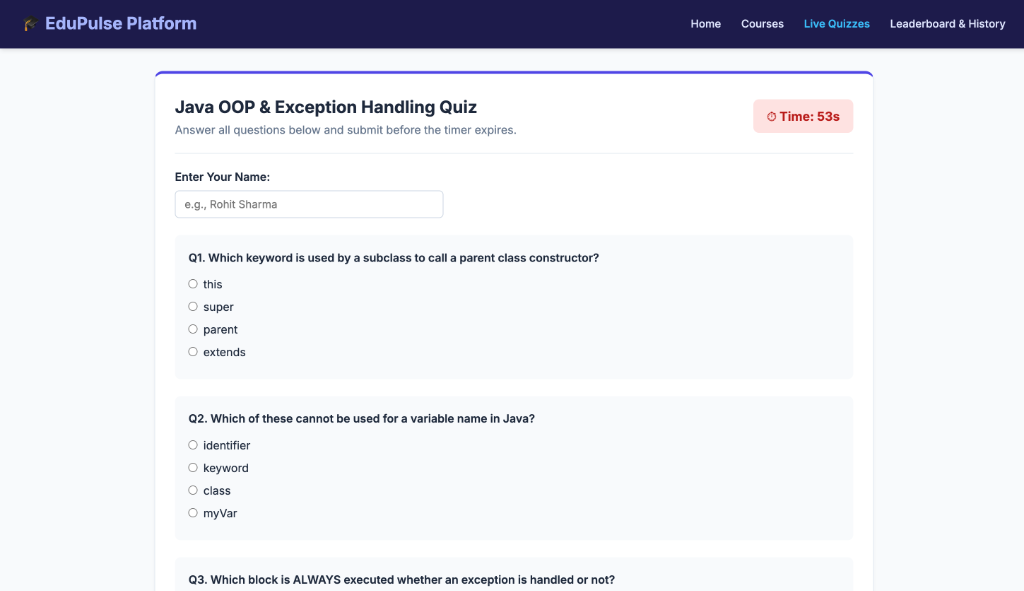
\includegraphics[width=0.92\textwidth]{images/home.png}
    \caption{EduPulse Home Portal (\texttt{http://localhost:8080/}) showcasing platform architecture.}
\end{figure}

\begin{figure}[H]
    \centering
    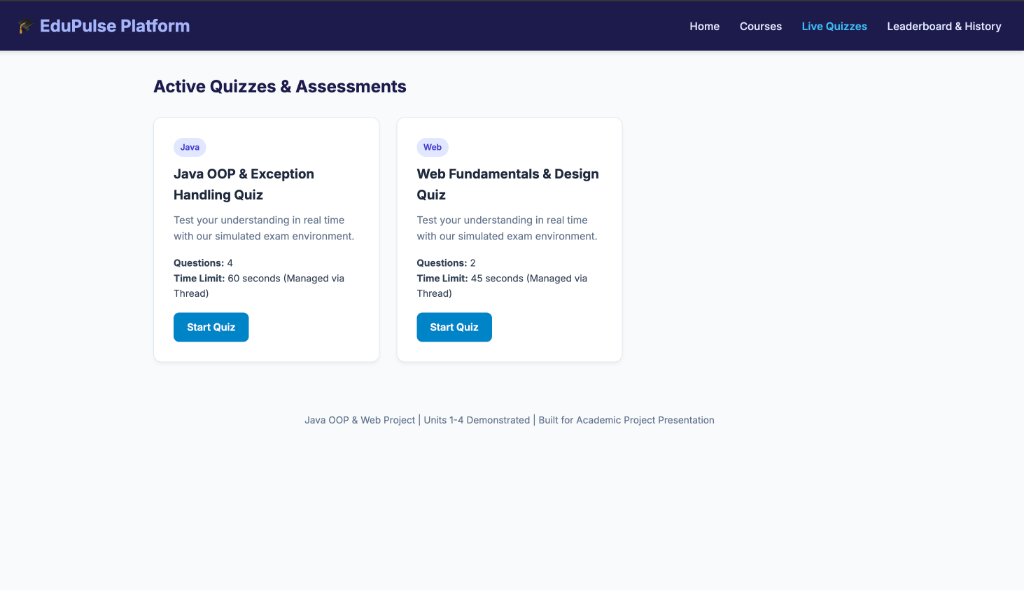
\includegraphics[width=0.92\textwidth]{images/courses.png}
    \caption{Courses Page (\texttt{/courses}) dynamically generated using Java \texttt{Course} objects.}
\end{figure}

\begin{figure}[H]
    \centering
    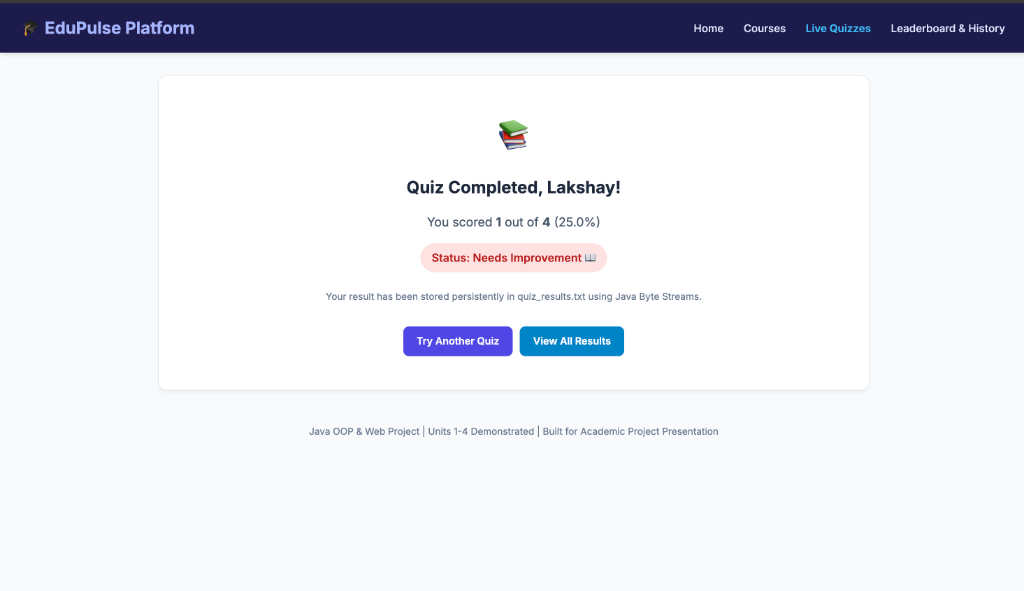
\includegraphics[width=0.92\textwidth]{images/quizzes.png}
    \caption{Quiz Assessment Catalog (\texttt{/quizzes}) displaying available exams.}
\end{figure}

% =========================================================================
% 7. CONCLUSION
% =========================================================================
\section{CONCLUSION}
The \textbf{EduPulse E-Learning Course \& Quiz Platform} fulfills all requirements of project-based learning for the course \textit{Object Oriented Programming with Java}. Concepts from Units 1 to 4 were successfully implemented and demonstrated both via terminal execution and a live web application.

% =========================================================================
% 8. REFERENCES
% =========================================================================
\section{REFERENCES}
\begin{enumerate}
    \item Herbert Schildt, \textit{Java: The Complete Reference}, 12th Edition, McGraw-Hill.
    \item Cay S. Horstmann, \textit{Core Java Volume I--Fundamentals}, 11th Edition, Prentice Hall.
    \item Oracle Corporation, \textit{Java Platform Standard Edition 17 API Specification}.
    \item GitHub Repository: \url{https://github.com/lakshay8toic/E-Learning-Course-Quiz-Platform}
\end{enumerate}

\newpage

% =========================================================================
% 9. APPENDIX: JAVA COURSE CERTIFICATES
% =========================================================================
\section*{APPENDIX: JAVA COURSE CERTIFICATES}
\addcontentsline{toc}{section}{APPENDIX: JAVA COURSE CERTIFICATES}

\begin{figure}[H]
    \centering
    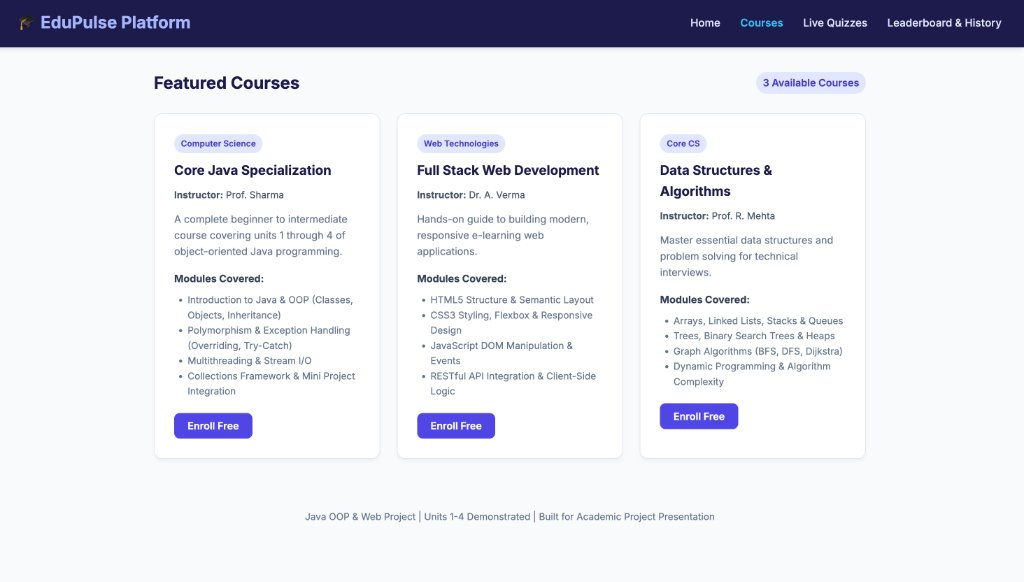
\includegraphics[width=0.88\textwidth]{images/cert_lakshay.jpg}
    \caption{Course Certificate: \textbf{Lakshay (AP24110010677)}, \textit{Java Development with Databases}, Coursera / SkillUp.}
\end{figure}

\vspace{1cm}

\begin{figure}[H]
    \centering
    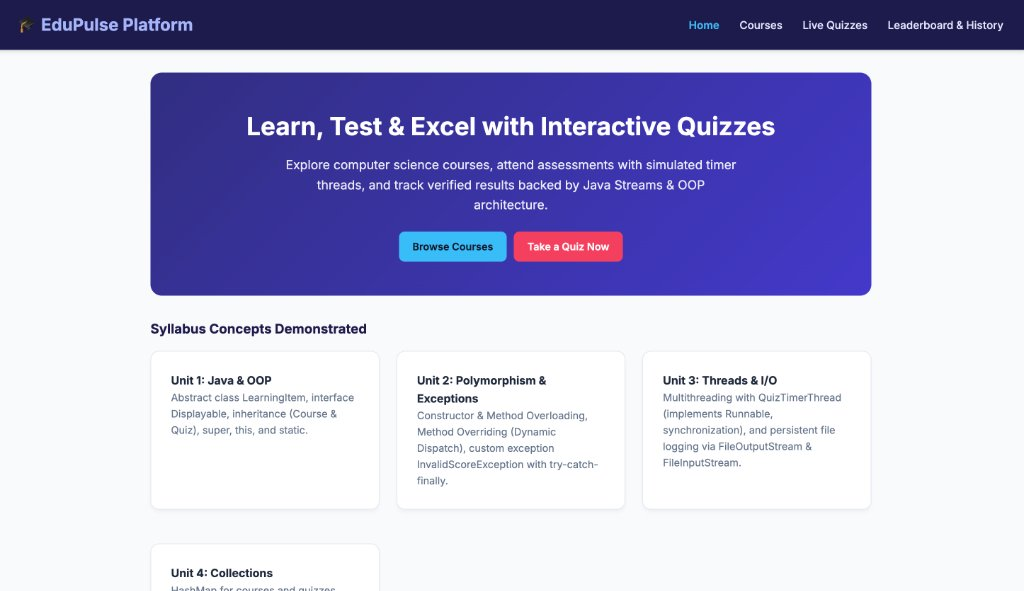
\includegraphics[width=0.88\textwidth]{images/cert_ahab.jpg}
    \caption{Course Certificate: \textbf{Md Ahab Firoz (AP24110011219)}, \textit{Java Development with Databases}, Coursera / SkillUp.}
\end{figure}

\end{document}
